\documentclass{article}
\usepackage{graphicx}
\usepackage{pgfplots}

\title{CUDA Grayscale Conversion Report}
\author{CHAPUIS Julien}
\date{\today}

\begin{document}

\maketitle

\subsection{CPU Implementation}
The CPU implementation converts the RGB image to grayscale using the following formula:
\[
\text{grayscale} = 0.2989 \times R + 0.5870 \times G + 0.1140 \times B
\]

\begin{figure}[h]
    \centering
    
\includegraphics[width=0.45\linewidth]{drunkCat.jpg}
    
\includegraphics[width=0.45\linewidth]{grayscaled_drunkCat.jpg}
    \caption{Original Cat Image (left) and Grayscaled Cat Image (right)}
    \label{fig:cat_images}
\end{figure}

\subsection{GPU Implementation}
The GPU implementation uses a CUDA kernel to perform the same conversion. The kernel is launched with a configurable number of threads per block.

\section{Experiment}
I experimented with different block sizes to measure the performance of the GPU. The block sizes tested were 32, 64, 128, 256, 512, and 1024.

\section{Results}
The following graph shows the execution time of the GPU implementation for different block sizes.

\begin{figure}[h]
    \centering
    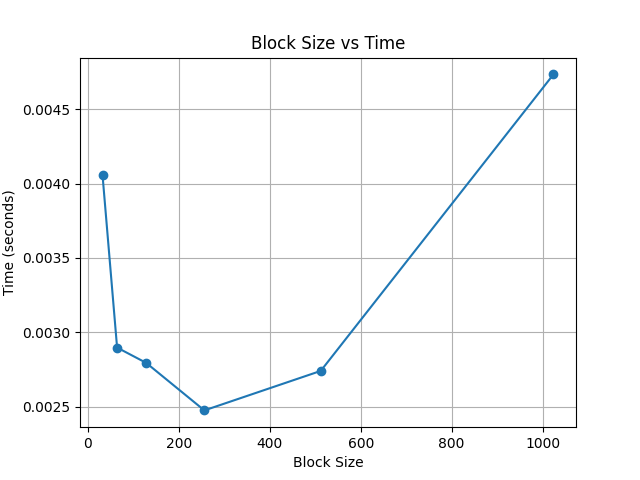
\includegraphics[width=\linewidth]{block_size_vs_time.png}
    \caption{Block Size vs Time}
    \label{fig:block_size_vs_time}
\end{figure}

\section{Discussion}
As shown in Figure \ref{fig:block_size_vs_time}, the execution time varies with different block sizes. The optimal block size for this specific implementation and hardware configuration can be identified from the graph though I don't understand why there's a peak for the last one.

\section{Conclusion}
The GPU outperforms the CPU implementation. The choice of block size has a noticeable impact on performance.

\end{document}